%!TEX TS-program = pdflatex
%!TEX root = progetto_finale.tex
%!TEX encoding = UTF-8 Unicode

\chapter{Implementazione}

Il linguaggio scelto per l'implementazione del progetto è Erlang. Esso è stato selezionato per diversi motivi tra cui: fornisce nativamente il supporto alla gestione di messaggi e scambio di essi tra diverse entità; permette di creare in poche righe di codice diversi beam a cui poter richiedere dei servizi; fornisce librerie tramite le quali è possibile creare facilmente gli automi e le interazioni fra essi. Inoltre supporta nativamente la programmazione concorrente semplificando la gestione da parte dello sviluppatore della programmazione parallela. Infine essendo un linguaggio funzionale, che quindi non presenta memoria condivisa, non permette l'esistenza della race condition tra processi.

In questo progetto non utilizzate piattaforme esterne di alcun genere poiché si assume che l'autenticazione tra utente e applicazione per il servizio sia già stata effettuata.

Essendo un'architettura peer to peer, non è necessaria alcuna piattaforma a parte l'autenticazione cliente - servizio.

\section{Generazione dell'ambiente virtuale}
Il problema della modellazione di una città è stato risolto con un grafo pesato connesso non orientato: si assume che se due nodi sono connessi è perché vi è una strada tra di essi ed è bidirezionale. Il peso indica quanto costa attraversarla. 

\subsection{Entità presenti}
Si immagina che i diversi nodi siano posizionati all'interno di un piano cartesiano, pertanto possiedono delle coordinate che ne indicano la posizione. Questo permette di capire la distanza tra di essi e quindi se diverse entità riescono a comunicare tra di loro.

\subsection{Componenti del grafo} \label{componenti_grafo_citta}
Ogni nodo del grafo possiede quattro proprietà:
\begin{itemize}
	\item attributo nome: generato del tipo ``aa'', ``ab'', ``ac'', ... incrementale per ogni nodo.
	\item attributo id: numero incrementale per ogni nodo a partire da 0. Utilizzato per la definizione del grafo della città.
	\item Coordinate X e Y: definiscono la posizione del nodo all'interno del piano cartesiano rappresentante la città.
\end{itemize}

Per quanto riguarda gli archi, essi posseggono tre proprietà:
\begin{itemize}
	\item ID\_Nodo\_1 - ID\_Nodo\_2: indica quali nodi collega.
	\item Peso: indica il peso dell'arco, calcolato in funzione della distanza tra i nodi che collega l'arco.
\end{itemize}

Infine vengono selezionati alcuni nodi tra quelli del grafo che conterranno le colonnine di ricarica. Per far questo è stato applicato il seguente algoritmo:
\begin{enumerate}
	\item In base al numero totale delle colonnine, il piano cartesiano viene suddiviso in parti uguali.
	\item Selezione di un nodo casuale all'interno della parte creata a cui assegnare la colonnina.
\end{enumerate}

\subsection{Parametri per la generazione}
Il linguaggio utilizzato per la generazione della città è python. All'interno del file ``map\_generator'' è possibile impostare i diversi parametri per la generazione della città, vale a dire:
\begin{itemize}
	\item WEIGHT\_MIN: Peso minimo degli archi.
	\item WEIGHT\_MAX:  Peso massimo degli archi.
	\item TOTAL\_NODES: Totale numero di nodi del grafo.
	\item TOTAL\_EDGES:  Totale numero di archi del grafo.
	\item TOTAL\_CHARGING\_COLS:  Totale numero delle colonnine di ricarica nel grafo.
	\item CARTESIAN\_SIDE:  Lato del quadrato cartesiano utilizzato per la mappa.
\end{itemize}

Per quanto riguarda il numero di colonnine, esso non è garantito essere rispettato per il seguente motivo: come spiegato precedentemente, l'algoritmo utilizzato suddivide il piano in parti uguali ma potrebbe capitare nel caso esse siano piccole che non vi sia alcun nodo all'interno. Dato che in ogni zona è presente al più una colonnina, può capitare che non siano presenti zone con nodi liberi a cui assegnare le rimanenti.

\subsection{File generati}
Lo script in python crea cinque file:
\begin{itemize}
	\item ``map.pdf'': I dati generati per il grafo vengono esportati nel formato dot e da esso viene generato questo file al cui interno è presente una rappresentazione visuale del grafo: sono presenti i nodi con le proprietà descritte precedentemente e gli archi con delle etichette rappresentanti il loro peso. Un esempio del pdf prodotto è l'immagine \ref{fig:esempio_citta_dot}.
	\item ``map.png'': Rappresentazione visuale delle posizioni dei nodi all'interno del piano cartesiano. I nodi colorati di rosso sono quelli contenenti le colonnine di ricarica. Un esempio del png prodotto è l'immagine \ref{fig:esempio_citta_png}.
	\item ``city\_map\_nodes.dat'': file testuale contenente i dati dei nodi formattati in modo da essere compatibili con la struttura creata in erlang. Un esempio è il seguente:
	\begin{lstlisting}
		10
		a 0 1 4
		b 1 2 12
		c 2 3 12
		d 3 3 16
		e 4 5 2
		...
	\end{lstlisting}
	\item ``city\_map\_graph.dat'': file testuale contenente i dati del grafo formattato in modo da essere compatibile con la libreria utilizzata in erlang. Un esempio è il seguente:
	\begin{lstlisting}
		10 30 undirected d
		6 0 17
		0 1 12
		1 8 18
		8 4 20
		4 7 14
		7 3 21
		3 9 18
		...
	\end{lstlisting}
	\item ``city\_map\_charging\_cols.dat'': file testuale contenente i dati dei nodi delle colonnine. Essi sono formattati in modo da essere compatibili con la struttura creata in erlang. Lo stile è il medesimo del file ``city\_map\_nodes.dat''.
	
\end{itemize}

\begin{figure}[htbp]
	\centering
	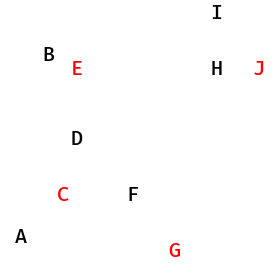
\includegraphics[width=8cm]{esempio_citta_png.jpg}
	\caption{Esempio del posizionamento dei nodi all'interno della città.}
	\label{fig:esempio_citta_png}
\end{figure}

\begin{figure}[htbp]
	\centering
	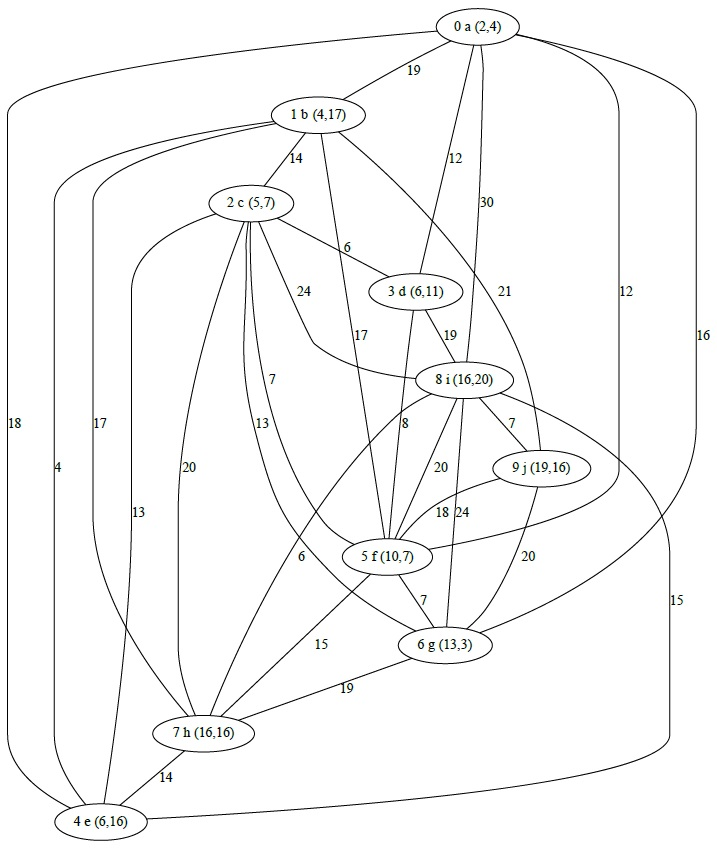
\includegraphics[width=14cm]{esempio_citta_dot.jpg}
	\caption{Esempio di grafo utilizzato per la simulazione della città.}
	\label{fig:esempio_citta_dot}
\end{figure}

\section{Entità Ambiente}
Questa entità, chiamata anche ``environment'', rappresenta il mondo in cui avviene la simulazione. Tramite esso è possibile creare entità, rimuoverle e far acccadere eventi.

\subsection{Variabili di stato}
Il suo stato contiene:
\begin{itemize}
	\item cars: lista dei pid delle macchine attualmente presenti nella città. In particolare è memorizzato il pid dell'automa ascoltatore, poichè è ad esso che vengono poi indirizzati i messaggi che riguardano la macchina di cui fa parte.
	\item total\_cars: numero totale delle macchine presenti. Esso viene aggiornato a ogni aggiunta e rimozione.
	\item users: lista dei pid degli utenti presenti nella città. Essa viene aggiornata sia quando l'utente viene creato che rimosso, vale a dire quando è giunto a destinazione.
	\item total\_users: numero totale degli utenti attualmente in città.
	\item cars\_crashed: lista delle macchine attualmente in stato ``crash''.
	\item total\_cars\_crashed: numero totale delle macchine in stato ``crash''.
	\item city: dati della città come descritti nella parte \ref{citta_e_algoritmi}.
	\item pid\_gps\_server: pid del server gps. Ne viene spiegato il funzionamento al punto \ref{gps_server}.
	\item autoEvents: flag che indica se gli eventi automatici sono abilitati oppure no.
	\item tick\_s\_pid: pid dell'istanza tick server dedicata all'environment.
	\item tick\_counter: contatore dei tick ricevuti.
	\item car\_pids: dizionario che associa il nome al pid delle macchine presenti.
	\item last\_car\_id: numero incrementale utilizzato per la generazione del nome delle macchine.
	\item user\_pids: dizionario che associa il nome al pid degli utenti present.
	\item last\_user\_id: numero incrementale utilizzato per la generazione del nome degli utenti.
	\item car\_prefix: prefisso utilizzato per i nomi delle macchine. Nella simulazione è pari a ``c''.
	\item user\_prefix: prefisso utilizzato per i nomi delle macchine. Nella simulazione è pari a ``u''.
\end{itemize}

\subsection{Eventi e gestione di essi}\label{env_events}
Sono stati gestiti sette tipi di eventi. Di seguito l'identificativo dell'evento ed il relativo nome assieme a una minima spiegazione:
\begin{itemize}
	\item -1 Nothing: nulla, lo stato della città resta inalterato.
	\item 1 Spawn car: questo evento causa la creazione di una macchina in un punto casuale della città. La creazione viene discussa nella parte \ref{creazione_distruzione_entita}.
	\item 2 Spawn user: questo evento causa la creazione di un utente in un punto casuale della città con una destinazione random. Maggiori informazioni sono presenti nella parte \ref{creazione_distruzione_entita}
	\item 3 Change target: quando occorre questo evento un utente casuale oppure quello passato per parametro cambierà la propria destinazione se possibile.
	\item 4 Car crash: una macchina scelta casualmente o determinata dal parametro passato passerà dallo stato normale a crash. Maggiori informazioni nella parte \ref{usersInQueue}. Il suo pid viene aggiunto alla lista ``cars\_crashed''. Nel caso venga selezionata una macchina già in quello stato viene stampato un messaggio di errore.
	\item 5 Car fix: una tra le macchine presenti nella ``lista cars\_crashed'' viene selezionata e ripatata tramite l'apposito evento. 
	\item 6 Remove Car: una macchina in stato ``idle'' viene rimossa dalla mappa. Se la macchina selezionata non è in idle si cerca una seconda macchia e via via fino al valore limite della variabile globale ``max\_kill\_tries''. Questo limite è dovuto alla volontà di evitare situazioni di stallo.
\end{itemize}

Nel caso in cui il flag ``autoEvents'' dello stato sia impostato a ``true'', il contatore dei tick ricevuti inizierà ad accumulare il tempo trascorso. In base alla variabile globale ``ticks\_event'' vengono determinati ogni quanti tick ricevuti debba acccadere un evento casuale tra quelli appena discussi.

Tramite le API fornite dal modulo è possibile innescare un determinato evento tramite la funzione ``triggerEvent'' e l'identificativo dell'evento desiderato. In alternativa è possibile utilizzare le funzioni già pronte per gli eventi a cui si può passare i parametri desiderati. Maggiori informazioni sono presenti nella documentazione dei singoli metodi.

\subsection{Creazione ed eliminazione delle entità} \label{creazione_distruzione_entita}
La creazione l'eliminazione di una determinata entità comportano diverse modifiche allo stato dell'environment, pertanto verranno analizzate in modo separato.

Dopo aver creato un'entità è necessario aggiornare il relativo contatore per evitare che esistano entità diverse ma con lo stesso nome.

\subsubsection{Creazione di una macchina}
I dati di cui necessita una macchina sono: posizione di partenza, pid del server gps a cui poter comnicare la propria posizione, mappa della città per poter eseguire l'algoritmo di elezione ed infine nome a lei assegnato. Dopo aver preparato i dati viene eseguita una chiamata al modulo della macchina e il pid ottenuto viene aggiunto alla lista delle macchina attualmente in città. Vengono incrementati i contatori delle macchine in città e dei nomi di esse. Infine viene aggiornato il dizionario che tiene traccia dell'associazione nome-pid macchina.

Il modulo della macchina crea le proprie istanze come spiegato al punto \ref{automaAscoltatore}.

\subsubsection{Creazione di un utente}
I dati di cui necessita un utente sono: posizione di partenza, richiesta di trasporto formata dalle due posizioni di partenza e arrivo, pid del server gps per la propria applicazione e nome dell'utente. Il pid del server gps serve poichè è l'automa utente a creare l'automa ``app\_utente''. Il punto di partenza della richiesta deve essere lo stesso della posizione iniziale dell'utente. In caso contrario viene generato un messaggio di errore. Come per la macchina, anche dopo la creazione dell'utente vengono aggiornate le relative liste.

\subsubsection{Eliminazione di una macchina}
Come già accennato nella parte \ref{env_events}, l'eliminazione di una macchina dall'ambiente avviene solo se essa si trova nello stato di idle. Questa scelta è stata fatta perché simile alla realtà. Una volta individuata, le si invia il segnale di morte e la si rimuove dalla lista delle macchine nell'ambiente. Inoltre viene rimossa la sua coppia nome-pid nel dizionario.

\subsubsection{Rimozione di un utente dall'ambiente}
Quando un utente è giunto a destinazione, esso considera compiuto il proprio dovere ed invoca il metodo dell'environment ``removeUser'' che ne elimina i riferimenti dallo stato come già spiegato per la macchina.

\section{Automi} \label{implementazioneAutomi}
Per l'implementazione degli automi è stata utilizzato ``gen\_statem'', il behavior erlang che semplifica la costruzione di macchine a stati finiti guidate da eventi. Questo behavior è un framework con numerose primitive riguardanti questi costrutti: invio e ricezione di eventi sincroni o asincroni, impostazione di timer e molto altro. Gli automi discussi in \ref{automi} sono stati implementati in modo relativamente veloce potendosi concentrare quasi esclusivamente sulla logica del loro funzionamento piuttosto che sui dettagli implementativi, nascosti appunto dal suddetto framework. 
Qui di seguito si riporta un link alla documentazione ufficiale del framework: \url{https://erlang.org/doc/man/gen_statem.html}.

I sorgenti sono stati opportunatamente commentati per descrivere il funzionamento del codice ma è opportuno compiere una descrizione generale di questi automi, soffermandosi sulle scelte implementative effettuate.

Gli automi implementati rispettano fedelmente gli schemi mostrati \ref{automi}, fatta eccezione per alcune mancanze e piccole modifiche che verranno ora elencate

\begin{itemize}
	\item Negli schemi progettuali si mostrava come la comunicazione fra automi interni a un'automobile non avvenisse mai in modo diretto, infatti l'ascoltatore del mezzo si comportava da proxy fra i due automi. Questa scelta progettuale è stata rivista in fase di implementazione, infatti si è ritenuto più veloce permettere una comunicazione diretta, ottenendo anche un codice più snello, pulito e dal comportamento più chiaro. 
	La comunicazione fra un automa interno al veicolo e un automa esterno, come per esempio fra l'automa dell'elezione e l'applicazione utente, avviene tuttavia usando l'ascoltatore come proxy, il quale infatti è l'interfaccia col mondo esterno per un veicolo. Questo ha permesso di diminuire le dipendeze fra i diversi automi: un automa esterno al mezzo deve conoscere soltanto l'ascoltatore per poter comunicare con il veicolo e tutte le sue istanze.
	\item Negli schemi progettuali erano stati inseriti molti stati che non presentano una controparte nel codice, questi erano stati definiti in fase di progettazione per chiarire le idee sui comportamenti degli automi, o per rendere gli schemi più espressivi, ma non si è ritenuto utile o conveniente inserirli nella loro implementazione. Il comportamento degli automi non è stato tuttavia intaccato dall'eliminazione di questi stati. 
	\item Similmente agli stati, alcuni eventi riportati negli schemi non presentano una controparte ``esatta'' negli automi, nel senso che i nomi di questi eventi sono stati ridefiniti in fase implementativa trovando alternative più espressive o, in generale, migliori per le esigenze del codice. Anche in questo caso il comportamento non è stato intaccato ed è possibile trovare un isomorfismo fra i nomi degli eventi inseriti negli schemi e quelli inseriti nel codice.
	\item Per la temporizzazione, in fase di progettazione, si faceva riferimento all'uso di orologi interni, i quali scandivano il tempo attraverso l'uso dei più volte citati ``Tick''. Questo è stato implementato con il modulo gestione tempo come mostrato al punto \ref{modules}, tuttavia per alcuni particolari casi si è preferito utilizzare i timer del behavior ``gen\_statem''. La scelta effettuata dipende dal particolare caso ma gran parte del codice usa i Tick per la temporizzazione.
\end{itemize}

\subsection{Struttura generale} \label{strutturaGeneraleAutomi}
I diversi automi implementati presentano tutti uno stato interno, inteso come una propria memoria che varia durante l'esecuzione, ed è importante non confondersi con lo stato della macchina a stati finiti, la similitudine fra i due termini si presta a diversi fraintendimenti e d'ora in poi si userà il termine ``memoria'' per indicare lo stato con questa accezione. La memoria di ogni automa è stata modellata definendo un record specifico, il quale aggrega tutti i dati necessari.

Il codice dei diversi automi è organizzato con una struttura molto simile che si può schematizzare in queste 5 sezioni:

\begin{enumerate}
	\item Codice per l'importazione di metodi da moduli esterni,importazioni di costanti definite esternamente, esportazione di metodi, definizione di costanti utilizzate solo localmente.
	\item definizione del record specifico per l'automa: secondo quanto detto ne modella la sua memoria.
	\item elenco dell'API dell'automa: inteso come le funzionalità della sua interfaccia, esportate per essere usate da altri automi.
	\item funzioni dell'automa: ricalcano gli stati dell'automa e i possibili comportamenti a seguito della ricezione dei vari eventi, ogni funzione inserita in questa sezione rappresenta una combinazione stato automa-evento ricevibile in quello stato, la logica dell'automa è raccolta in questa sezione.
	\item funzioni interne: usate localmente.
\end{enumerate}

Ogni automa nel codice ha questa suddivisione e i file col codice sono stati opportunatamente marcati con dei commenti per enfatizzare questa struttura. Ulteriori commenti sono stati disposti nel codice per semplificarne la comprensione, in particolar modo sono stati definiti dei contratti nei metodi delle API.

\subsection{Eventi Globali - la funzione ``handle\_common''} \label{eventiGlobaliAutomi}
In questa sezione si descrive come sono stati gestiti gli eventi globali negli automi, ossia eventi che possono essere ricevuti in stati diversi dell'automa. Come descritto sopra, la sezione 4 del codice raccoglie le funzioni che descrivono la logica dell'automa, il behavior ``gen\_statem'' e il pattern matching di Erlang garantiscono che, se l'automa si trova in un certo stato e riceve un particolare evento, verrà eseguita la funzione insrita in questa sezione che rappresenta la particolare combinazione stato-evento; questa, eventulamente, modificherà la memoria del processo e/o  effettuerà un cambiamento di stato. 
Qui viene riportato un frammento di codice che mostra una di queste funzioni: 

\begin{lstlisting}
waiting_car_queued(cast, taxiServingYou, State) ->
	{next_state, waiting_car, State};
\end{lstlisting}

Si noti come il secondo parametro della funzione indichi il nome dell'evento che ``triggera'' l'esecuzione del codice, mentre il nome della funzione indica lo stato.

Gli eventi globali portano a un ovvio overhead se implementati in questo modo, infatti per un evento ricevibile in N stati è necessario scrivere N funzioni diverse, se il comportamento è lo stesso in tutti gli stati questo comporta la scrittura di N funzioni tutte uguali ottenendo ulteriormente numerose dipendeze.

Grazie alle comode primitive Erlang si può definire una sola funziona che gestisca lo stesso evento per stati diversi, nel progetto in esame questa è stata chiamata ``handle\_common''. Nella sezione 4 di quasi tutti gli automi, in testa, sono state definite diverse funzioni ``handle\_common'' che adempiono, appunto, a questo scopo. Ne viene qui riportato un esempio;

\begin{lstlisting}
%ricezione del comando di terminazione
handle_common(cast, {die}, _OldState, State) ->
	PidGpsModule = State#appUserState.pidGPSModule,
	gps_module:end_gps_module(PidGpsModule),
	gen_statem:stop(self());
\end{lstlisting}

Queste funzioni hanno una firma diversa in base all'evento: l'atomo inserito come secondo parametro della funzione indica quale evento ``triggera'' l'esecuzione di quel codice.

\section{Automi Macchina} \label{automiMacchina}

le macchine, come mostrato negli schemi progettuali, presentano più automi che lavorano in parallelo: automa ``ascoltatore'', automa ``gestione movimento'', ``gestione batteria'' ed ``elezione''. La descrizione sommaria di questi è già stata affrontata in \ref{automi}, in questa sezione verrà fatta una descrizione di essi soffermandosi sugli aspetti principali della loro implementazione.

\subsection{Automa ascoltatore} \label{automaAscoltatore}

L'automa ascoltatore, o listener, è il padre della gerarchia che rappresenta i vari automi del mezzo. Quando l'environment genera un nuovo taxi si preoccupa soltanto di inizializzare un automa di questo tipo, il quale automaticamente creerà tutti i restanti automi sottostanti mantenendo un riferimento a ognuno di essi nella propria memoria. Oltre ad essi, l'ascoltatore si impegna a creare anche il modulo gps usato dall'auto e il ``server tick'', indicando ad esso di inserire fra gli abbonati tutti gli automi del mezzo, così da garantire una temporizzazione sincronizzata. Se l'environment è interessato a provocare qualche evento che intacca i taxi, comunica soltanto con questo automa, il quale poi comunicherà con gli opportuni automi sottostanti.

\subsubsection{Lista di utenti in coda} \label{usersInQueue}

Per semplificare la gestione di incidenti, cambi di destinazione, cambiamenti alla topologia della mappa cittadina, si è pensato di mantenere nell'ascoltatore una lista di tutti gli utenti in coda per il taxi. In particolare, è stato definito uno speciale record che rappresenta una ``comanda'' del taxi, ossia una istanza di richiesta del servizio da parte di un utente.
Questo record è definito nel sorgente di questo automa e si chiama ``userInQueue'', esso presenta questi 3 campi:

\begin{enumerate}
	\item pid = il pid dell'applicazione dell'utente richiedente il servizio
	\item position = la posizione attuale del cliente 
	\item target = la destinazione del cliente
\end{enumerate}

Nella propria memoria, un ascoltatore, mantiene una lista di record di questo tipo, uno per ogni cliente in coda.
Nel caso in cui accadano gli eventi sopra citati, tale lista viene consultata in questi modi:
\begin{itemize}
	\item incidente: per ogni elemento della lista, viene inviato al pid dell'applicativo la notifica di incidente.
	\item cambio di destinazione: viene fatto un controllo sulla lunghezza della lista, se questa presenta un solo elemento significa che c'è un solo utente accodato ed è possibile il cambio di desinazione, ne viene quindi calcolata la fattibilità in base alla batteria attuale. Se la lista presenta più elementi allora non è possibile il cambio e l'app dell'utente richiedente viene opportunatamente notificata.
	\item cambio di topologia: per ogni elemento della lista, viene calcolato se è possibile garantire quella comanda considerando il cambiamento appena avvenuto nei percorsi, notificando le relative app in base all'esito. Questo aspetto è stato trattato in \ref{aggiornamentoMappa}.
\end{itemize}

\subsubsection{Legame con automa elezione} \label{listenerElection}
Questo automa lavora a stretto contatto con l'automa dell'elezione, essi concorrono a garantire all'utente richiedente il servizio un giusto candidato. Quando l'ascoltatore riceve dall'utente la richiesta, oppure la partecipazione all'elezioni da altri taxi, inoltra all'automa elezione quest'ultima e attende il processamento dell'algoritmo distribuito. Al termine dell'esecuzione di questo algoritmo, l'ascoltatore riceve uno specifico evento contenente l'ouptut, come spiegato nel punto \ref{implementazione_algoritmo_elezione}: in esso è presente il riferimento al taxi vincitore e se questo combacia con se stesso significa che il taxi si dovrà spostare verso nuovi nodi. Questo comporta un aggiornamento della lista dei punti da visitare, aspetto che verrà affrontato nelle prossime sezioni quando si parlerà dell'automa gestione movimento.

\subsection{Automa batteria} \label{automaBatteria}
Questo automa si proccupa di controllare il livello della batteria del mezzo, controllando se questa è inferiore o superiore a certi valori di soglia e in base ai casi notificare il mezzo se è necessario andare a ricaricare oppure se non è più necessario continuare la ricarica.

Inoltre, questo automa controlla se il mezzo è stazionario da un lungo intervallo di tempo e in tal caso lo notifica riguardo alla necessità di iniziare la ricarica con pannelli solari. Questa forma di ricarica è più lenta di quella con colonnina ma è stata implementata in modo da evitare casi di stallo del veicolo. Infatti, un taxi potrebbe rimanere fermo su un nodo, impossibilitato a vincere nuove elezioni a causa di una batteria troppo bassa. 

\subsection{Automa gestione movimento} \label{automaMoving}

Questo automa si preoccupa di garantire lo spostamento del mezzo, l'automa ascooltatore invia ad esso le tappe da percorrere secondo quanto detto in \ref{listenerElection}.
Per tappa si intende dire uno spostamnto fra due nodi adiacenti. Concettualmente questo automa ha o scopo di consumare le tappe ricevute dall'esterno e notificare il suo ascoltatore di avvisare eventuali utenti incontrati nel percorso o serviti. 

le tappe sono state modellate creando un record chiamato, per l'appunto, ``tappa'', che presenta questi 4 campi:

\begin{enumerate}
	\item user = pid dell'applicazione utente che viene servito in questa tappa
	\item type = il tipo di nodo che verrà raggiunto dopo questa tappa, si è deciso di definire 4 diversi tipi di nodi, vedasi sezione successiva ``tipi di nodi''
	\item t = il tempo necessario a percorrere questa tappa
	\item node\_name = il nome del nodo raggiunto dalla tappa
\end{enumerate}
Sono stati definiti opportuni metodi che elaborano l'output dell'algoritmo del calcolo dei percorsi minimi e creano le tappe formattate in questo modo, pronte per essere date in pasto a questo automa.

\subsubsection{Tipi di nodi} \label{tipiTappe}

assumiamo che un utente abbia sottomesso al servizio una richiesta di questo tipo: spostamento dal nodo ``a'' al nodo ``d''.
i tipi di nodi delle tappe sono stati distinti con questi 4 atomi:

\begin{enumerate}
	\item 'user\_start' = indica il nodo nel quale si trova l'utente, il nodo ``a'' della richiesta
	\item 'user\_target' =  indica il nodo che l'utente vuole raggiungere, il nodo ``d'' della richiesta
	\item 'intermediate' =  indica un nodo intermedio, ossia tutti quei nodi che nel tragitto da percorrere si frappongono fra il nodo ``a'' e il nodo ``d'' della richiesta oppure fra il nodo ``d'' e quello della colonnina da raggiungere, eventualmente, per la ricarica.
	\item column = indica il nodo contenente la colonnina di ricarica, verso il quale andare eventualmente a caricare dopo aver servito l'utente.
\end{enumerate}

\subsubsection{Consumo delle tappe} \label{consumo tappe}
Questo automa raccoglie i record tappe in una lista nella propria memoria, dopo un numero fissato di tick ``consuma'' la  tappa inserita in testa, elaborandone il contenuto per sapere come comportarsi, alcuni esempi: il tipo della tappa indica se è necessario comunicare all'utente aggiornamenti sulla sua richiesta oppure se è stata raggiunta la colonnina di ricarica, il valore 't' indica il tempo rimanente al raggiungimento del prossimo nodo.
Le possibili combinazioni di comportamenti in base al contenuto della tappa sono molte, una lista esaustiva di tutti questi non è lo scopo di questo documento e sono stati riportati solo alcuni esempi per favorire la comprensione dell'automa.

\subsubsection{Ricarica del mezzo} \label{tappe colonnina}
Come detto in \ref{tipiTappe}, uno dei tipi di tappa è quello del nodo con la colonnina di ricarica, pertanto l'automa deve inserire tra le sue mansioni anche lo spostamento verso le colonnine e la ricarica del mezzo.

Questo automa riceve dall'automa ascoltatore 2 liste di tappe: quelle da consumare per soddisfare la richiesta del cliente e quelle da consumare per raggiungere la colonnina di ricarica. Alla ricezione di queste l'automa procede al consumo della prima lista, ma salva la seconda in un attributo specifico della memoria non sapendo se consumerà anche queste tappe. Se, durante lo spostamento, la batteria scenderà sotto un certo livello, l'automa batteria invierà a questo la notifica secondo quanto detto in \ref{automaBatteria} e l'automa si accingerà al consumo della seconda lista. 
In tale modo si garantisce che venga seguito il percorso verso la colonnina solo se viene valutato necessario caricare il mezzo.

Al raggiungimento del nodo 'column' l'automa si sposta nello stato di ricarica, nel quale a ogni intervallo costante di tick aumenta la propria batteria. Questo processo continua fino alla ricezione della notifica di fermo da parte dell'automa batteria, con la quale avviene il ritorno allo stato idle.
Similmente, se l'automa batteria decide di avviare la ricarica solare, l'automa compie le stesse transizioni.

\subsubsection{Dati necessari all'elezione}
I dati necessari all'algoritmo di elezione riguardano principalmente il processamento di elementi presenti nella memoria di questo automa, si pensi per esempio al livello di batteria rimanente oppure al nodo destinazione verso cui il mezzo si sta dirigendo per soddisfare l'ultimo cliente in coda.
Per tale motivo si è valutato utile inserire nell'API di questo automa un metodo che restituisca tutti questi dati necessari all'automa dell'elezione, il quale lo chiamerà quando necessario per l'esecuzione dell'algoritmo. Il metodo è stato chiamato ``getDataElection'' e restituisce valori diversi a seconda dello stato del taxi, viene qui riportato quello eseguito del caso in cui questo automa si trovi in idle :

\begin{lstlisting}
idle({call,From}, {getDataElection}, State) ->
	Cost_To_last_Target = 0,
	Current_Target = State#movingCarState.currentPos,
	Battery_level = State#movingCarState.batteryLevel,
	Packet = {Cost_To_last_Target, Current_Target, Battery_level ,ok},
	{keep_state, State, [{reply,From,Packet}]};
\end{lstlisting}

\section{Automi Utente} \label{automiUtenti}
Gli automi degli utenti sono più semplici di quelli dei taxi, si suddividono in automa utente e applicazione utente. 

\subsection{Automa utente}
L'automa utente, similmente a quello ascoltatore per i taxi, genera il suo automa applicazione utente con il quale comunica per usare il servizio e ricevere notifiche su di esso. L'environment, quando genera un nuovo utente, si preoccupa di inizializzare un automa di questo tipo e l'app verrà generata indipendentemente. 
Non c'è molto da dire su questo automa, l'environment comunica con questo automa per immettere nuove richieste al sistema o cambiare la destinazione di un utente e l'applicazione inoltra ogni aggiornamento sulla gestione della richiesta al rispettivo automa utente.

\subsection{Automa applicazione}
L'automa applicazione utente genera, al momento della inizializzazione, il proprio modulo gps per poter conoscere il taxi più vicino a cui inviare la richiesta. 

\subsubsection{Timer}
Questo automa è uno dei pochi che usano i timer del behavior piuttosto che il server tick per la temporizzazione. Il timer usato è di tipo ``state\_timout'' (uno specifico timer del behavior). 
Questo timer viene lanciato quando l'app invia al taxi più vicino la richiesta di spostamento e si sposta nello stato ``waiting\_election'', nella quale aspetta una risposta. Se questa risposta non viene ricevuta nei tempi impostati dal timer, quest scatta e l'app decide di reiterare la richiesta. 

\subsubsection{Attese random}
ci sono 4 cirocstanze in cui l'app decide di aspettare un tempo random e reiterare la richiesta dell'utente al taxi più vicino:
\begin{enumerate}
	\item l'applicazione non ha trovato nessun taxi nei paraggi per inviare la richiesta, ossia il modulo gps non ha rilevato nessuna macchina nella mappa.
	\item c'è stato un incidente del mezzo nel quale viaggiava l'utente.
	\item il taxi a cui è stata inviata la richiesta è occupato nell'esecuzione di un'altra elezione.
	\item il pacchetto contenente l'output dell'elezione ricevuto dal taxi indica che non è presente nessun vincitore.
\end{enumerate}


\section{Mappa città e relativi algoritmi} \label{citta_e_algoritmi}
Il record ``city'' contiene cinque parametri:
\begin{itemize}
	\item city\_graph: grafo caricato dalla libreria descritta al punto \ref{libreria_algoritmi}.
	\item total\_nodes: numero totale dei nodi del grafo.
	\item total\_edges: numero totale di archi del grafo.
	\item nodes: nodi presenti nella mappa secondo la struttura definita al punto \ref{nodi_citta}.
	\item column\_positions: sottoinsieme dei nodi che contengono le colonine.
\end{itemize}

Esso contiene lo stato attuale della città dal punto di vista topologico. Le sue componenti vengono utilizzate da diverse entità del sistema per diversi scopi:
L'automa elezione inserire riferimento ne utilizza il city\_graph per calcolare i costi della macchina.

L'entità ambiente inserire riferimento ne utlizza i nodi per generare casualmente le posizion iniziali di macchine e utenti.

Il Gps Server \ref{gps_server} ne utilizza i nodi per creare la propria struttura dove tiene traccia della posizione attuale delle entità presenti in un determinato istante nella città

\subsection{Nodi città}\label{nodi_citta}
Come già descritto al punto \ref{componenti_grafo_citta}, ogni nodo possiede diverse proprietà che vengono memorizzate nell'apposito record definito in questo modo:
\begin{itemize}
	\item name: nome del nodo
	\item id: identificativo numerico del nodo, utlizzato per la sua codifica nel grafo. Questo è necessario poichè la libreria descritta al punto \ref{libreria_algoritmi} per identificare i nodi utilizza il loro id numerico.
	\item pos\_x: coordinata sull'asse delle ascisse del nodo.
	\item pos\_y: coordinata sull'asse delle ordinate del nodo.
\end{itemize}

All'avvio l'entità ambiente, tramite il modulo ``node\_utils'', carica la lista dei nodi presenti nel file ``city\_map\_nodes.dat'' e la lista presente nel file ``city\_map\_charging\_cols.dat''. Queste due liste vengono utilizzate per identificare quali sono i nodi della città e quali di essi sono colonnine. 

La scelta di separarle è stata effettuata poichè nella ricerca della colonnina più vicina alla posizione della macchina è sufficiente calcolare la distanza tra ogni colonnina e il punto desiderato, senza scorrere tutti i nodi della mappa.

Il metodo ``get\_nearest\_col/3'' presente nel modulo ``city\_map'' permette di sapere quale colonnina sia quella più geograficamente vicina al nodo passato come parametro.

Il modulo ``node\_utils'' fornisce i diversi getter per ottenere le informazioni desiderate a partire dalla lista e un identificativo per un determinato nodo. Esso inoltre fornisce dei metodi per ottenere un nodo random presente, con la possibilità di escludere un nodo. Questa proprietà viene utilizzata nella generazione delle richieste degli utentei come spiegato al punto REF\_CREATING\_REQUEST.

\subsection{Libreria per algoritmi} \label{libreria_algoritmi}
Data la natura del progetto, è necessario poter gestire grafi ed applicare ad essi l'algoritmo di Dijkstra per il calcolo dei cammini minimi tra due nodi di esso. Per eseguire questo compito, si è scelto di utilizzare la libreria ``erlang-algorithms'' fornita da Aggelos Giantsios, reperibile al sito \url{https://github.com/aggelgian/erlang-algorithms}. Essa fornisce sia le strutture base che gli algoritmi da applicare ad esse.

Di questa libreria vengono principalmente tre funzionalità:
\begin{itemize}
	\item graph:from\_file/1: permette, leggendo un file, di crearne il grafo associato in un'apposita struttura erlang.
	\item dijkstra:run/2: esegue l'algoritmo di dijkstra applicato al grafo passato come parametro iniziando dal nodo indicato.
	\item graph\_utils:getDataPath/2: vengono passati i risultati calcolati da dijkstra e il nodo target di cui si vuole sapere il percorso calcolato.
\end{itemize}

L'algoritmo di Dijkstra viene utilizzato nell'automa dell'elezione come spiegato al punto REF\_elezione\_automa.

\section{Moduli Gps e Server Gps}
Il problema in esame concerne la posizione delle diverse entità all'interno di una città, pertanto è necessario esse possiedano un modulo in grado di dir loro la posizione e distanza delle altre entità presenti. Per far questo è stato deciso di creare due moduli:
\begin{itemize}
	\item gps\_server: tiene traccia delle posizioni di tutte le entità.
	\item gps\_module: comunica con il server per sapere quali sono le entità vicine a lui.
\end{itemize}

\subsection{Gps Server}\label{gps_server}
Con lo scopo di simulare la ricezione dei vicini delle diverse entità, esso fornisce dei messaggi tramite i quali è possibile ottenere queste informazioni. Questo modulo utlizza quattro record:

\begin{itemize}
	\item nodeDistance: è una tupla formata da due valori, vale a dire ``dist'', che indica la distanza dal nodo che fa la richiesta, e ``entities'', che è una lista di pid. Il significato di essa è ``a questa distanza ci sono queste entità''.
	\item entity: è una tupla formata da tre valori: ``pid'', ossia il pid dell'entità, ``type'', l'atomo che contiene l'informazione sul tipo di entità, ed infine ``position'', che contiene il nome del nodo dov'è attualmente situata l'entità.
	\item nodeEntities: contiene due campi, vale a dire ``nodeData'', che contiene i dati del nodo che si sta considerando (dati come definiti al punto \ref{nodi_citta}), e ``entities'', che è una lista di pid. 
	\item gpsServerState: contiene due liste, una di entity come appena definite e una di nodeEntities.
\end{itemize}

Le funzionalità che offre il server sono principalmente due:

\begin{itemize}
	\item getNearEntities/2: i parametri che riceve sono la posizione di partenza e la potenza del segnale. Ciò che il server fa è il calcolo della distanza di tutti i nodi della mappa dal nodo di partenza e filtra questi in base al valore della potenza del segnale. Non importa l'ordine, l'output è una lista contenente i nodi entro il range che il segnale copre.
	\item getSortedEntities/2: i parametri che riceve sono la posizione di partenza e la potenza del segnale. Il server, dopo aver calcolato la distanza di tutti i nodi e filtrati in base alla distanza massima, li ordina tramite un algoritmo di sorting. L'output è una lista di pid ordinati in base alla distanza dal nodo di partenza ma senza l'informazione della distanza. Sta al richiedente estrarre il pid voluto.
\end{itemize}

In entrambi i casi vengono effettuati i seguenti passaggi: nel calcolo delle distanze, viene creata un'istanza del record ``nodeDistance'' contenente, come già spiegato, distanza e pid presenti nel nodo; poichè i pid delle entità sono presenti in liste diverse, viene applicata la funzione ``packNodes'' che estrae dal record ``nodeDistance'' i pid e ne crea una lista.

\subsection{Gps Module}\label{gps_module}
Rappresenta il modulo ``localizzatore vicini'' descritto nella parte \ref{modules}. Esso fornisce all'automa della macchina e dell'applicazione dell'utente le funzioni per il recupero delle entità vicine.

Il suo stato contiene i seguenti parametri:
\begin{itemize}
	\item pid\_entity: il pd a cui è associato il modulo gps. Nel protetto corrisponde all'applicazione dell'utente oppure all'automa ascoltatore della macchina.
	\item name\_entity: il nome dell'entità di cui fa parte.
	\item pid\_gps\_server: il pid del server gps a cui fare le richieste delle entità vicine.
	\item entity\_type: tipo dell'entità a cui è associato. Nel caso faccia parte di una macchina esso sarà ``car'' mentre nel caso dell'applicazione utente sarà ``user''.
	\item current\_position: nome del nodo attuale dov'è situata l'entità di cui fa parte.
	\item module\_range: potenza del segnale gps del modulo. Viene utilizzato dal gps server per filtrare i risultati come già spiegato al punto \ref{gps_server}.
	\item map\_side: poiché viene assunto che il modulo dell'applicazione utente possa sempre individuare la macchina più vicina, la potenza utilizzata dalla funzione ``getNearestCar'' è pari alla diagonale della mappa, pertanto sicuramente individua tutte le macchine.
\end{itemize}

La funzione ``getNearestCar'' richiede al Gps server le entità presenti ordinate secondo la distanza dal nodo dov'è situato il modulo gps e, dopo aver rimosso il pid relativo a alla propria entità, ne seleziona il primo elemento. 

La funzione ``getNearCars'' esegue come la precedente la richiesta al server indicando la propria posizione e il proprio livello di segnale. La risposta del server, dopo aver rimosso da essa il pid relativo all'entità di cui il modulo fa parte, viene inoltrata all'entità che ha eseguto questa funzione.


\section{Automa Elezione}
Il principale problema affrontato in questo progetto è stato quello di eleggere quale sia la migliore macchina per soddisfare la richiesta dell'utente. Come già accennatto precedentemente al punto \ref{automiMacchina}, ogni macchina possiede un'istanza di questo automa.

\subsection{Record utilizzati}\label{record_elezione}
Per l'elezione vengono utilizzati diversi record, che per lo più rispecchiano i pacchetti definiti al punto \ref{descrizione_pacchetto}.

\begin{itemize}
	\item user\_request: formato dalla coppia ``from''  e ``to'' indica il punto di partenza e arrivo dell'utente.
	\item dataElectionBegin: creato dall'automa ascoltatore, indica all'elezione di iniziare i calcoli per l'elezione. Al suo interno contine la richiesta dell'utente ed il pid dell'applicazione dell'utente.
	\item dataElectionPartecipate: creato dall'automa elezione, rispecchia la struttura spiegata precedentemente. Contiene: riferimento alla macchina ``padre'' per la successiva comunicazione dei risultati; user request come definita prima; ttl per determinare se inoltrare ulteriormente l'invito.
	\item electionCostData: vengono creati da ogni macchina e contengono il proprio pid per l'eventuale comunicazione del vincitore assieme al CC e CRDT come definiti al punto \ref{funzioni_di_costo_macchine}.
	\item carPartecipate: formato da tre campi, ha lo scopo di mantenere le informazioni dei nodi invitati a partecipare a una determinata elezione. Contiene il pid della macchina invitata, una lista dei costi ad essa associata ed una variabile ``sent results'' che indica se la determinata macchina ha già inviato oppure no i propri calcoli per l'elezione.
	\item election\_result\_to\_car: risultati per la macchina, contengono il pid del vincitore, il pid dell'app dell'utente per la creazione delle relative tappe per l'automa moving e la richiesta in modo che sia più facile popolare la lista ``users in queue'' dell'automa ascoltatore. Maggiori informazioni al punto REF\_USERS\_IN\_QUEUE.
	\item election\_result\_to\_user: risultati per gli utenti, vengono creati dall'automa ascoltatore risultato vincitore dell'elezione. Contengono il pid e nome del taxi vincitore assieme al tempo di attesa per l'arrivo nella posizione dell'utente.
\end{itemize}

\subsection{Varaibli di istanza dell'automa}\label{stato_elezione_automa}
Ogni istanza dell'automa possiede alcune variabili costanti e altre che variano per ogni elezione. Queste sono le variabili comuni a tutte le elezioni:
\begin{itemize}
	\item pidCar: pid dell'ascoltatore della macchina, utilizzata per inviare i messaggi agli altri automi.
	\item nameCar: nome della macchina, utilizzata per i messaggi di stato.
	\item pidMovingCar: pid dell'automa moving, a cui vengono richiesti i dati dell'elezione come discusso al punto REF\_DATI\_ELEZIONE.
	\item pidGps: pid della propria scheda gps, utilizzata per sapere quali siano le macchine vicine.
	\item cityMap: mappa della città, come descritta al punto \ref{citta_e_algoritmi}.
\end{itemize}

Di seguito le variabili utilizzate localmente per un'unica elezione:
\begin{itemize}
	\item flag\_initiator: indica se è questa la macchina iniziatrice dell'elezione, vale a dire quella che dovrà calcolare chi sia il miglior taxi.
	\item pidAppUser: nel caso del nodo iniziatore, si tiene il riferimento all'utente che ha richiesto il trasporto per la successiva comunicazione.
	\item currentRequest: copia della richiesta dell'utente, utilizzata per la generazione del record ``election\_result\_to\_car''
	\item my\_election\_cost: costi calcolati per la macchina che possiede l'elezione. Nel caso essa risulti candidabile equivalgono a una lista contenente i ``electionCostData'' definiti precedentemente, altrimenti una lista vuota.
	\item queueToManage: è una tupla formata da tre campi, i quali sono la coppia costo totale - percorso relativi ai diversi path che la macchina deve compiere per soddisfare un cliente. Sono i dati ``grezzi'' ottenuti dall'applicazione degli algoritmi sui grafi, da elaborare per l'automa moving.
	\item dataToSendPartecipate: è il record ``dataElectionPartecipate'' utilizzato come invito alla partecipazione per gli altri automi elezione.
	\item parent: pid dell'automa che svolge il ruolo di padre durante l'elezione. 
	\item carsInvited: lista dei pid delle macchine invitate alla partecipazione dell'elezione da parte di un determinato modo
	\item childrenPartecipate: elenco di record ``carPartecipate'' che consente di tener traccia dei nodi che partecipano effettivamente all'elezione.
	\item totalCosts: lista dei costi dei nodi figli di un determinato nodo e di quello del nodo corrente.
	\item car\_moving\_queue\_data: elenco dei record creati a partire dalla ``queueToManage'' per l'automa moving.
\end{itemize}

\subsection{Algoritmo di Elezione}\label{implementazione_algoritmo_elezione}
Riprendendo l'algoritmo definito al punto \ref{algoritmo_elezione}, di seguito ne viene analizzata l'implementazione di ogni passo.

\begin{itemize}
	\item Il nodo inizatore riceve dall'automa ascoltatore il messaggio che contiene le informazioni necessarie per l'elezione. 

	\lstinline|{beginElection, dataElectionBegin}|

	Esso quindi calcola i propri costi come spiegato al punto \ref{implementazione_calcolo_costi} e dopo aver richiesto al proprio modulo gps quali siano le entità vicine, aggiorna il proprio stato. Nel caso in cui la lista delle macchine vicine non sia vuota, le invita e si sposta nello stato ``initiator\_final\_state''. Nel caso invece in cui ci siano delle macchine da invitare, prepara il record ``dataElectionPartecipate'' impostando le variabili e il ttl come descritto nella variabile globale ``max\_hops\_election'', lo invia alle macchine da invitare con l'apposito messaggio e si sposta in ``running\_election''.

	\lstinline|{partecipateElection, Data}|
	\item I nodi che ricevono l'invito di partecipazione possono essere di due tipi: nello stato ``idle'' e in un altro stato dell'elezione. Nel primo caso rispondono al nodo che li ha invitati con il messaggio 

	\lstinline |{invite_result, {Self_Pid, i_can_join}}|
	
	per indicare che partecipano attivamente all'elezione. Calcolano i propri costi secondo il metodo \ref{implementazione_calcolo_costi} e controllano il ttl contenuto nell'invito. Nel caso in cui sia maggiore di zero chiedono al modulo gps i propri vicini e inviano loro il messaggio di invito con ttl diminuito di un'unità. Nel caso sia uguale a zero non estendono l'invito di partecipazione. Successivamente si spostano nello stato ``running\_election'' in attesa delle risposte dei nodi invitati. Nel caso invece il nodo sia in uno stato non di ``idle'' è l'ascoltatore ad inviare al nodo richiedente il messaggio

	\lstinline |{invite_result, {Self_Pid, i_can_not_join}}|

	ad indicare la non partecipazione.

	Nel caso non sia necessario l'invito di altre macchine all'elezione, dallo stato idle ci si sposta nello stato ``waiting\_final\_results'' in attesa della comunicazione del vincitore dal parte del nodo iniziatore.
	\item Nello stato ``running\_election'' ogni automa gestisce le due liste precedentemente definite ``carsInvited'' e ``childrenPartecipate''. 
	
	Ogni volta che un nodo in questo stato riceve un messaggio del tipo 
	
	\lstinline |{invite_result, {Self_Pid, Result}}|
	
	cerca il pid ``Self\_Pid'' dalla lista ``carsInvited'' e se lo trova ed il valore della variabile ``Result'' è pari a ``i\_can\_join'' crea un record del tipo ``carPartecipate'' con il campo ``sent\_results'' a ``not\_sended\_results''. Nel caso in cui esso non venga trovato vuol dire che il nodo ha già mandato i propri risultati e quindi è già stato rimosso dalla lista degli invitati.

	Ogni volta che un nodo in questo stato riceve un messaggio del tipo 

	\lstinline |{costs_results, Data}|

	Controlla se il nodo è ancora presente nella lista degli invitati. In caso affermativo lo rimuove, crea il record ``carPartecipate'' con i dati ricevuti e impostando il flag ``sent\_results'' a ``ok'' aggiungendolo alla lista dei partecipanti attivi definita prima. Nel caso in cui non sia presente nella lista degli invitati, lo cerca nella seconda lista e ne aggiorna le proprietà utilizzando come identificativo il pid del nodo.

	In entrambi i casi alla fine viene chiamata la procedura dedicata al calcolo della fine ``running\_election'' che se, la lista degli invitati è vuota e tutti i partecipanti hanno inviato i propri dati, invia i dati al nodo genitore e sposta l'automa nello stato di attesa / calcolo dei risultati dell'elezione.
	
	Per ridurre i calcoli eseguiti da un unico nodo, si è optato per inoltrare al genitore solamente i dati del nodo migliore del proprio sottoalbero. I dati scambiati contenenti le informazio di un particolare nodo sono presenti nei record di tipo ``electionCostData'' come già definito.

	\item Il nodo iniziatore, a differenza dei nodi partecipanti, appena riceve tutte le risposte dai propri figli si sposta nello stato speciale ``initiator final state'' nel quale, dopo l'applicazione della funzione di selezione del miglior dato, crea i risultati dell'elezione. In base ai calcoli effettuati crea il record del vincitore e inoltra il messaggio a tutti i nodi partecipanti all'elezione.
	
	\item Ogni nodo partecipante inoltra il pacchetto winner ricevuto a tutti i nodi presenti nella lista ``childrenPartecipate''. Questo perché sono essi coloro che hanno effettivamente partecipato all'elezione, non è detto siano tutti quelli invitati.

	\item Oltre all'inoltro del messaggio vincitore, ogni nodo controlla se è lui stesso il vincitore e, in caso positivo, prepara i record in modo compatibile con quelli dell'automa moving come spiegato al punto \ref{automaMoving}.

	\item Infine inoltra i risultati al proprio ascoltatore e torna nello stato dell'elezione ``idle'' dopo aver reimpostato le proprie variabili legate alle elezioni.
\end{itemize}

\subsection{Calcolo dei costi per l'elezione}\label{implementazione_calcolo_costi}
Per calcolare i costi di una determinata macchina si sono utilizzate le formule descritte al punto \ref{funzioni_di_costo_macchine}. Dopo aver richiesto i dati attuali all'automa moving della macchina tramite la funzione ``getDataElection'', viene calcolato il nodo della mappa dove è presente una colonnina di ricarica più vicino al punto di arrivo della richiesta in esame.
In totale si calcola il costo di tre percorsi: dalla posizione della macchina dopo l'eventuale trasporto in corso fino al punto di prelievo del cliente richiedente; il tragitto del cliente; il percorso tra punto obiettivo del cliente e nodo dove è presente la colonnina.
Si procede quindi con il calcolo dei percorsi aggiungendo via via i costi calcolati e calcolando se la batteria rimanente è sufficiente. Nel caso in cui durante il calcolo di uno di essi la batteria risulti insufficiente si considera che la macchina non possa essere vincitrice.

La procedura ``calculateSelfCost'' restituisce due tipi di risultati:
\begin{lstlisting}
	{-1, -1, i_can_not_win, {}}
\end{lstlisting}
quando viene calcolato la macchina non possa vincere l'elezione.

\begin{lstlisting}
	{CC, CRDT, i_can_win, QueueCar}
\end{lstlisting}
quando viene calcolato la macchina può vincere l'elezione. La variabile QueueCar viene salvata nello stato della macchina assegnandola alla ``queueToManage'' e utilizzata dopo come già spiegato.

\subsection{Gestione dei timer}
Lo scopo è di gestire il caso in cui un nodo non risponda alle richieste dell'elezione...